\chapter{Reconhecimento de voz}
\label{cap:speech-recognition}

Neste capítulo, abordaremos a parte teórica do reconhecimento de voz, sem nos preocuparmos com a forma de implementação ou sua aplicação no contexto deste trabalho. Em particular, analisaremos brevemente os principais parâmetros que influenciam seu uso.

% ---------------------------------------------------------------------

\section{Definição}

\textbf{Reconhecimento automático de voz} (ou da fala), muitas vezes referido como \textit{speech to text} (\textbf{STT}), é um campo multidisciplinar que envolve as áreas de Inteligência Artificial, Estatística e Linguística. Busca-se desenvolver metodologias e tecnologias para que computadores sejam capazes de captar, reconhecer e traduzir a linguagem falada para texto \citep{sttDefinition}.

% ---------------------------------------------------------------------

\section{História}

Apresentamos uma breve visão histórica de sistemas de reconhecimento de voz, baseado principalmente em \citep{STTHistory}, desde seu início até os dias atuais.

% ---------------------------------------------------------------------

\subsection{Décadas de 50 e 60: Primeiros passos}

O primeiro sistema de reconhecimento de voz conhecido foi o \textit{Audrey}, construído em 1952 por três pesquisadores do \textit{Bell Labs}. A máquina conseguia reconhecer apenas dígitos falados por um único usuário.

10 anos depois, a IBM apresentou o \textit{Shoebox}, que reconhecia 16 palavras em inglês, entre elas os dígitos de 0 a 9. Quando captava palavras como \textit{plus}, \textit{minus} ou \textit{total}, \textit{Shoebox} instruía outra máquina de adições a realizar cálculos ou imprimir o resultado. A entrada era feita por um microfone (figura \ref{shoebox}), que convertia a voz do usuário em impulsos elétricos, classificados internamente por um circuito de medição \citep{shoebox}.

\begin{figure}[H]
  \centering
  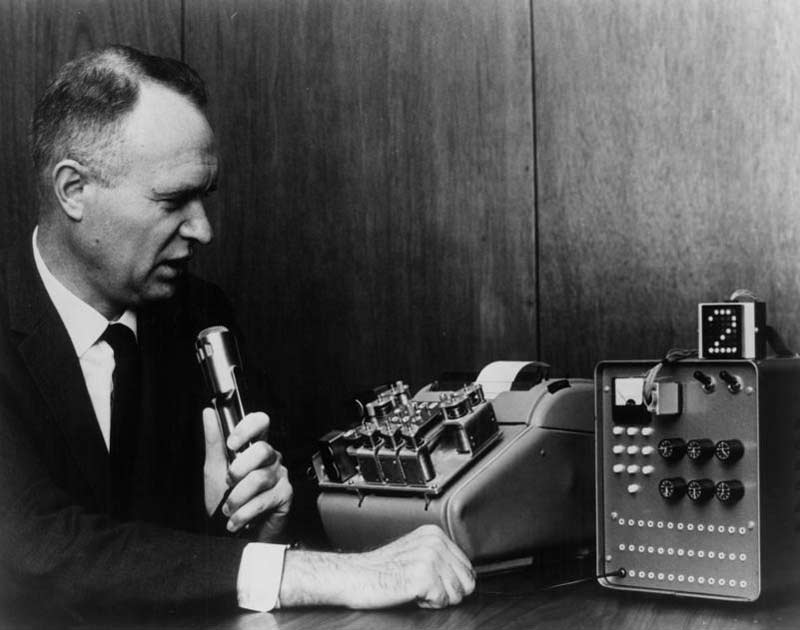
\includegraphics[width=.5\textwidth]{image/shoebox.jpg}
  \caption{Máquina \textit{Shoebox} sendo operada \citep{shoeboxImage}}
  \label{shoebox}
\end{figure}

Laboratórios nos EUA, URSS, Inglaterra e Japão começaram a desenvolver hardware para reconhecer uma maior variedade de sons. Conseguiu-se suporte para quatro vogais e nove consoantes; um avanço notável, considerando a tecnologia da época.

% ---------------------------------------------------------------------

\subsection{Décadas de 70 e 80: Grandes avanços}

Na década de 70, o departamento de defesa dos EUA mostrou grande interesse em financiar a tecnologia de reconhecimento de voz. Tal impulso ajudou no desenvolvimento do sistema \emph{Harpy} de reconhecimento de voz pela Universidade Carnegie Mellon.

Usava-se um grafo para representar o domínio das palavras reconhecíveis. Um algoritmo de busca heurística, \emph{Beam Search}, era aplicado para procurar a melhor interpretação para a voz de entrada. Este algoritmo assemelha-se ao \textit{Best-First Search} (BFS), que explora um grafo através da expansão do estado mais promissor ao sair do estado presente. No entanto, sua otimização consiste em ordenar os próximos possíveis estados, através de uma heurística, antes de realizar uma expansão, o que permite prever o quão longe o estado presente está em relação ao estado meta. Com isso, o \textit{Beam Search} é caracterizado como um algoritmo guloso, que gasta menos memória quando comparado ao BFS \citep{beamSearch}.

Através de uma forma de busca mais eficiente, \textit{Harpy} conseguia entender 1011 palavras, aproximadamente o vocabulário de uma criança típica de três anos.

Sistemas de reconhecimento de voz só tiveram um avanço realmente significativo na década de 80, devido a um método estatístico denominado \textbf{Modelo Oculto de Markov} (ou \textbf{HMM}, sigla para \textit{Hidden Markov Model}). Ao invés de procurar por modelos de palavras em padrões de som, considera-se a probabilidade de um som desconhecido possuir palavras, o que acelerou o processo e tornou possível usar um vocabulário maior nos computadores. Veremos HMM com um pouco mais de detalhe no capítulo \ref{cap:hmm}.

Outro modelo que ganhou bastante popularidade na mesma época foi o de redes neurais, que é efetivo para classificar palavras isoladas e fonemas individuais mas encontra problemas em tarefas envolvendo reconhecimento contínuo. Ao contrário do HMM, este método não consegue modelar bem dependências temporais. No entanto, em ambos os casos, existia a necessidade de falar pausadamente para o sistema poder melhor interpretar o usuário.

Os progressos em sistemas de reconhecimento de voz começaram a se refletir no meio comercial. Destacamos a boneca \textit{Julie} (figura \ref{julie}), comercializada em 1987 como \textit{``Finalmente, a boneca que te entende''}, pois era capaz de ser treinada para responder à voz de uma criança.

\begin{figure}[H]
  \centering
  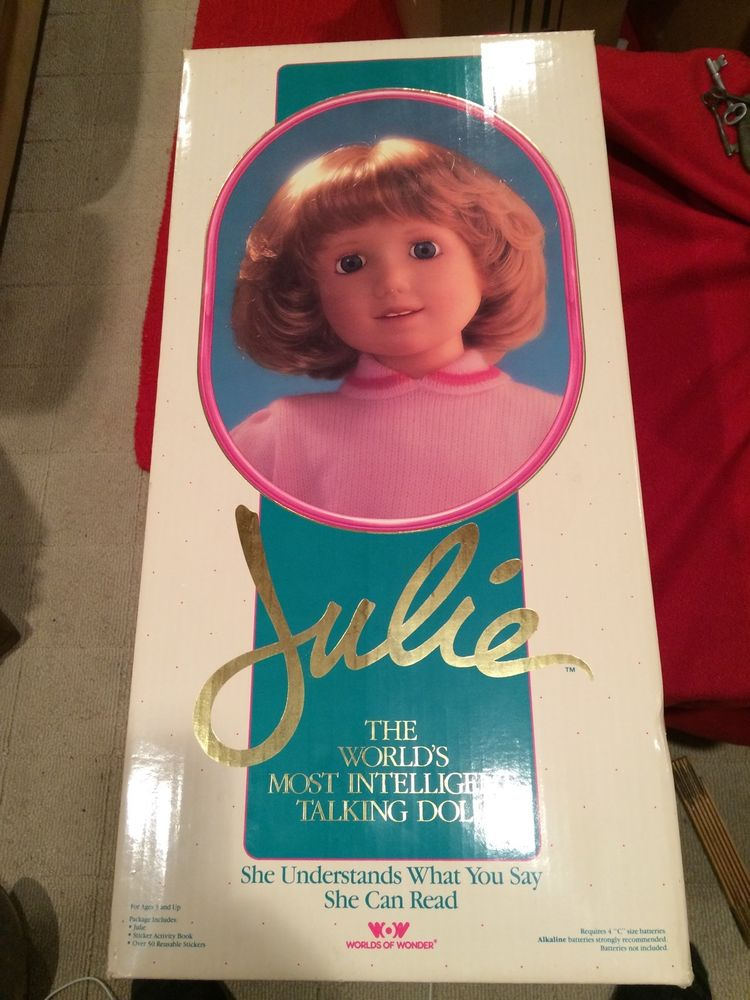
\includegraphics[width=.35\textwidth]{image/julie.jpg}
  \caption{Caixa da boneca \textit{Julie}; note, na parte inferior, a frase \textit{``Ela entende o que você diz''} \citep{julieImage}}
  \label{julie}
\end{figure}

% ---------------------------------------------------------------------

\subsection{Década de 90 até hoje: Popularização}

Na década de 90, a popularização de computadores para uso pessoal e o desenvolvimento de processadores mais rápidos permitiu que o reconhecimento de voz ficasse viável para uma quantidade maior de pessoas.

Em 1996, surgiu o primeiro portal de voz, \emph{VAL}, criado pela empresa de telecomunicações norte-americana BellSouth. O sistema atendia chamadas telefônicas e respondia de acordo com a informação proferida pelo cliente.

Até o final dos anos 2000, sistemas de reconhecimento de voz pareciam ter ficado estagnados em uma acurácia de aproximadamente 80\%, e muitas aplicações eram caracterizadas pela complexidade ou dificuldade de uso se comparadas ao tradicional \textit{mouse} e teclado.

A popularidade do conceito ressurgiu com força através do aplicativo de Busca por Voz, feito pela Google para iPhone. As duas razões para o sucesso dessa forma de busca eram a facilidade de entrada de dados, se comparado ao teclado da plataforma, e o uso de \textit{data centers} em nuvem da Google, o que retirava a necessidade de um poderoso processamento nos iPhones em si. Com isso, mostrava-se que era possível contornar duas das principais limitações: a disponibilidade de dados e a dificuldade de processá-los eficientemente.

A evolução na tecnologia de reconhecimento de voz foi tamanha que, atualmente, é inegável seu impacto em nosso dia a dia. Um celular moderno consegue captar palavras ou pequenas frases de seu usuário dentre um enorme vocabulário para fazer buscas na Internet, tocar uma música ou fazer uma ligação. Alguns países chegam até a usar reconhecimento de voz para autenticar a identidade de alguém por telefone, com o objetivo de evitar fornecer dados pessoais pelo mesmo. Também há usos em transportes, na área médica e para fins educativos, muitas vezes acentuados pela maior facilidade em se falar um comando comparado ao uso de um teclado ou interface gráfica.

% ---------------------------------------------------------------------

\section{Componentes de um sistema genérico}
\label{sttComponents}

A figura \ref{generic-stt} apresenta os três componentes de um sistema genérico envolvendo STT \citep{sttComponentsParameters}:

\begin{itemize}
\item O \textbf{usuário} do sistema, que codifica um comando através de sua voz;

\item O \textbf{dispositivo} de STT, que converte a mensagem falada para um formato interpretável;

\item O \textbf{software de aplicação}, que recebe a saída do dispositivo e realiza uma ação apropriada.
\end{itemize}

\begin{figure}[H]
  \centering
  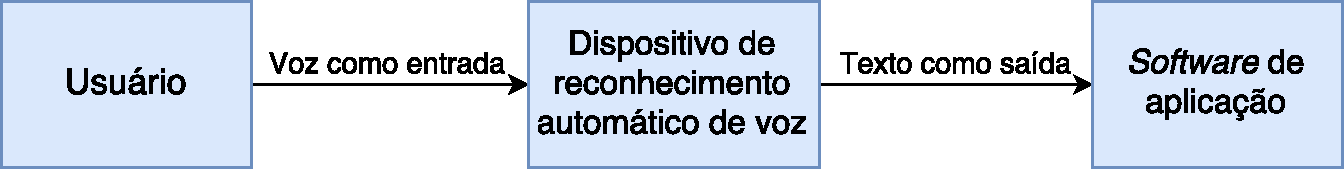
\includegraphics[width=.9\textwidth]{image/generic-stt.pdf}
  \caption{Sistema genérico de reconhecimento automático de voz \citep{sttComponentsParameters}}
  \label{generic-stt}
\end{figure}

% ---------------------------------------------------------------------

\section{Principais termos}

De acordo com \citep{sttComponentsParameters} e \citep{sttBasics}, apresentamos, a seguir, os termos mais recorrentes em sistemas de reconhecimento de voz. Também entramos em detalhes nos tipos de parâmetros que caracterizam as capacidades de um sistema de reconhecimento de voz, influenciando sua forma de funcionamento, eficiência e acurácia. A influência destes fatores varia de acordo com o tipo de aplicação que se deseja construir.

% ---------------------------------------------------------------------

\subsection{Fluência}

A fluência está relacionada à forma de se comunicar com o sistema. Tipicamente, a fala do usuário pode ser feita através de \emph{palavras isoladas}, com pausas entre elas; \emph{palavras conectadas}, que são concatenadas sem pausas; ou \emph{fala contínua}, onde o fluxo de palavras é semelhante a uma fala natural.

% ---------------------------------------------------------------------

\subsection{Dependência do usuário}

A dependência ou não do usuário classifica os sistemas em dois grupos:

\begin{itemize}
\item Os sistemas \textbf{dependentes} (\textit{speaker-dependent}), caracterizados pelo \emph{treinamento} feito pelo usuário. Isto é, são computadores que analisam e se adaptam aos padrões particulares da fala captada, resultando em uma maior acurácia. Geralmente, o usuário deve ler algumas páginas de texto para a máquina antes de começar a usar o sistema. Esta variante é comumente usada em casos particulares, onde um número limitado de palavras deve ser reconhecido com bastante precisão \citep{speakerDependency}.

\item Os sistemas \textbf{independentes} (\textit{speaker-independent}), que são desenvolvidos para reconhecer a voz de qualquer pessoa e não requerem treinamento. É a melhor opção para aplicações interativas que usam voz, já que não é viável fazer com que os usuários leiam páginas de texto antes do uso, ou para sistemas usados por diferentes pessoas. Sua desvantagem é a acurácia menor se comparado ao reconhecimento dependente; para contornar isso, costuma-se limitar o vocabulário reconhecido pelo sistema \citep{speakerDependency}.
\end{itemize}

% ---------------------------------------------------------------------

\subsection{Vocabulário}

O vocabulário representa as palavras reconhecidas pelo sistema. Seu tamanho pode ser pequeno (menor que 20 palavras) até muito grande (mais de 20 mil palavras), sendo diretamente proporcional à velocidade do reconhecimento. Além disso, a similaridade entre a pronúncia de algumas palavras pode afetar a acurácia, uma vez que a distinção entre elas torna-se mais complicada.

% ---------------------------------------------------------------------

\subsection{\textit{Utterance}}

O termo \textit{utterance} não possui uma tradução exata no contexto de reconhecimento de voz, embora possa ser interpretado como \textit{``pronunciamento, elocução''}. Refere-se à vocalização (fala) de uma ou mais palavras, pronunciadas de forma contínua e terminando com uma pausa clara, que possuem um significado único ao computador. Em outras palavras, \textit{utterances} são o conteúdo entendido pelo sistema após receber a fala do usuário.

Ao voltarmos para o sistema genérico de reconhecimento de voz apresentado na seção \ref{sttComponents}, notaremos que a interpretação de \textit{utterances} representa a saída produzida pelo dispositivo de STT.

% ---------------------------------------------------------------------

\subsection{Parâmetros ambientais}

Parâmetros ambientais referem-se a fatores externos ao sistema que podem interferir no reconhecimento de voz. Destacam-se:

\begin{itemize}
\item A \textbf{relação sinal/ruído}, que avalia a intensidade média do sinal recebido em relação ao ruído de fundo, tipicamente medido em decibéis (dB). Quanto menor a taxa, maior a dificuldade no reconhecimento de voz.

\item O \textbf{próprio usuário}, o que inclui o volume de sua voz, a velocidade com que fala e até mesmo sua condição psicológica: o nível de estresse de um piloto sob ataque em uma aeronave é diferente de alguém simplesmente querendo ouvir uma música, por exemplo.
\end{itemize}
